\input ../talk-header.tex
\usepackage{centernot}
\usepackage[]{algorithm2e}

\title
{ML Week}
\subtitle{0x0A \hspace{2mm}  Recommendation}

% If you wish to uncover everything in a step-wise fashion, uncomment
% the following command: 
%\beamerdefaultoverlayspecification{<+->}

\begin{document}

\begin{frame}
  \titlepage
\end{frame}

%%%%%%%%%%%%%%%%%%%%%%%%%%%%%%%%%%%%%%%%%%%%%%%%%%%%%%%%%%%%%%%%%%%%%%
%\talksection{Break}

\begin{frame}
  \frametitle{Definition}

  \centerline{\parbox{.8\textwidth}{ Given data about a user, his
  environment, and some items of interest (\textit{training data}),
  determine items to recommend.}}

  \vspace{1cm}
  \only<2>{
    We don't have to find the $\max k$.

    It's enough to find $k$ within some $\max n$.
  }
\end{frame}

%% TODO -- lots of images

\begin{frame}
  \frametitle{Examples}
  \begin{itemize}
  \item Amazon
  \item Google News (or Le Monde)
  \item Facebook
  \item Medical testing
  \item App Store / Google Play
  \item Youtube
  \item Advertising
  \item Netflix, last.fm, Spotify, Pandora, \dots
  \item Browser (URL recommendations)
  \item Search
  \end{itemize}
  % TODO: images
\end{frame}

\begin{frame}
  \frametitle{Client Value Proposition}
  \begin{itemize}
  \item Find opportunities
  \item Reduce choice
  \item Explore options
  \item Discover long tails
  \item Recreation
  \end{itemize}
\end{frame}

\begin{frame}
  \frametitle{Provider Value Proposition}

  \begin{itemize}
  \item Offer a unique or additional service (beyond competitors)
  \item Customer trust and loyalty
  \item Increase sales, CTR, conversions
  \item Better understand customers
  \end{itemize}
\end{frame}

% ======================================================================
% Technique Overview

\begin{frame}
  \frametitle{Recommendation}

  \begin{tabular}{|p{5.7cm}|p{4cm}|}
    \hline
    \topstrut\hbox{Content-based filtering}
    \hbox{\it (filtrage basée sur le continu)}
    &
    More things similar to what I like\bottomstrut
    \\
    \hline
    \topstrut\hbox{Collaborative filtering}
    \hbox{\it (filtrage collaboratif)}
    &
    More of what other people who like what I like like
    \bottomstrut
    \\
    \hline
    \topstrut\hbox{Knowledge-based filtering}
    \hbox{\it (filtrage basée sur connaissance)}\bottomstrut
    &
    More of what I need.\bottomstrut
    \\
    \hline
  \end{tabular}
\end{frame}

\begin{frame}[t]
  \frametitle{Content-based filtering}
  \textit{\purple{More things similar to what I like}}\\
  \textit{\red{Plus de ce qui ressemle à ce que j'aime}}

  Pro
  \begin{itemize}
  \item [yes!] No need for community
  \item [yes!] Possible to compare items 
  \end{itemize}

  \bigskip
  Con
  \begin{itemize}
  \item [no] Understand content
  \item [yes] Cold start problem
  \item [no] Serendipity
  \end{itemize}
\end{frame}

\begin{frame}[t]
  \frametitle{Collaborative filtering}
  \textit{\purple{More of what other people who like what I like like}}\\
  \textit{\red{Plus de ce que d'autres qui aiment ce que j'aime aiment}}

  Pro
  \begin{itemize}
  \item [yes!] No need to understand content
  \item [yes!] Serendipity
  \item [yes!] Learn market
  \end{itemize}

  \bigskip
  Con
  \begin{itemize}
  \item [no] User feedback
  \item [yes] Cold start problem (users)
  \item [yes] Cold start problem (items)
  \end{itemize}
\end{frame}

\begin{frame}[t]
  \frametitle{Knowledge-based filtering}
  \textit{\purple{More of what I need}}\\
  \textit{\red{Plus de ce qu'il faut}}

  Pro
  \begin{itemize}
  \item [yes!] Deterministic
  \item [yes!] Certainty
  \item [no!] Cold start problem
  \item [yes!] Market knowledge
  \end{itemize}

  \bigskip
  Con
  \begin{itemize}
  \item [yes] Studies to bootstrap
  \item [yes] Static model, doesn't learn from trends
  \end{itemize}
\end{frame}


% ======================================================================
% Linear Algebra Basics

\begin{frame}[t]
  \frametitle{Utility Matrix}

  \begin{itemize}
  \item Users (utilisateurs)
  \item Items (objets)
  \end{itemize}

  \only<2->{The goal is to fill in the blanks.}

  \only<2>{
    \vspace{1cm}
    \centerline{\begin{tabular}{l|ccccc}
        & $I_1$ & $I_2$ & $I_3$ & $I_4$ & $I_5$ \\
        \hline
        $U_1$ & 1 & & & & \\
        $U_2$ & & & 1 & 1 & 1 \\
        $U_3$ & & 1 & & 1 & 1
      \end{tabular}}

    \bigskip
    \centerline{\gray{Example: books sales at Amazon.}}
  }
  \only<3>{
    \vspace{1cm}
    \centerline{\begin{tabular}{l|ccccc}
        & $I_1$ & $I_2$ & $I_3$ & $I_4$ & $I_5$ \\
        \hline
        $U_1$ & 3 & & & & \\
        $U_2$ & & & 5 & 1 & 4 \\
        $U_3$ & & 2 & & 5 & 1
      \end{tabular}}

    \bigskip
    \centerline{\gray{Example: film advice at Netflix.}}
  }

  \only<2->{
    \bigskip
    \gray{\it But thousands or millions of columns and rows.}
  }
\end{frame}

\begin{frame}
  \frametitle{Utility Matrix}

  How do we make the matrix?
  \begin{itemize}
  \item Ask users
  \item Observe users
  \end{itemize}

  That's usually expensive\dots
\end{frame}

\begin{frame}
  \frametitle{Item Profiles}

  Examples:
  \begin{itemize}
  \item Films \gray{$\qquad\Rightarrow$ ?}
  \item Books \gray{$\qquad\Rightarrow$ ?}
  \item News \gray{$\qquad\Rightarrow$ ?}
  \item Images \gray{$\qquad\Rightarrow$ ?}
  \end{itemize}

  \only<2>{\gray{ Films :}

    \gray{Content: acters, directors, year (decade, etc.), length}

    \gray{Collaborative: seen, opinion~(1--5), when seen relative to release}
  }
  \only<3>{\gray{Books:}

    \gray{Content : authers, genre, year (decade, etc.), number of pages, content (very difficult)}

    \gray{Collaborative: read, opinion~(1--5), how read}
  }
  \only<4>{\gray{News:}

    \gray{Content : source, section, TF-IDF word vectors}

    \gray{Collaborative: }
  }
  \only<5>{\gray{Images :}

    \gray{Content:}

    \gray{Collaborative:}
  }
  
  \only<6>{

    \gray{Also: user profile, user behavior}
  }

\end{frame}

\begin{frame}
  \frametitle{Mathematics}

  \vspace{1cm}
  \centerline{Vectors}

  \vspace{1cm}
  \centerline{Similarity}
\end{frame}

\begin{frame}
  \frametitle{Similarity : Jaccard Index}

  \only<1>{\green{or: \textit{Indice de Jaccard}, \textit{Jaccard similarity coefficient}}}
  
  \vspace{1cm}
  Similarity:
  \begin{displaymath}
    J(A,B) = \frac{|A\cap B|}{|A\cup B|}
  \end{displaymath}

  \only<2>{
    Distance:
    \begin{displaymath}
      J_{\delta}(A,B) = 1 - J(A,B)
    \end{displaymath}
  }
\end{frame}

\begin{frame}
  \frametitle{cosine similarity}

  \only<1>{\green{or: \textit{mesure cosinus}, \textit{Similarité cosinus}}}

  \vspace{1cm}
  Similarity:
  \only<1>{
    \begin{displaymath}
      \cos \theta = \frac{A\cdot B}{\parallel A\parallel \parallel B\parallel}
    \end{displaymath}
  }
  \only<2->{
    \begin{displaymath}
      S_C(A,B) = \frac{A\cdot B}{\parallel A\parallel \parallel B\parallel}
    \end{displaymath}
  }
  
  \only<3->{
    Distance:
    \begin{displaymath}
      D_C(A,B) = 1-S_C(A,B)
    \end{displaymath}
  }

  \only<4>{
    \gray{We only consider non-empty components in the vector.}
  }
\end{frame}

\begin{frame}
  \frametitle{Texts: TF-IDF}
  
  \begin{itemize}
  \item Vectors of word frequencies
  \item Frequency $\centernot\implies$ significance
  \item<2> Term Frequency - Inverse Document Frequency
  \end{itemize}
\end{frame}

\begin{frame}
  \frametitle{Texts: TF-IDF}

  \blue{
    \begin{displaymath}
      TF_{ij} = \frac{f_{ij}}{\max_k f_{kj}} \qquad\qquad
      IDF_I = \log_2\left( \frac{N}{n_i} \right)
    \end{displaymath}
  }
  \blue{
    \begin{displaymath}
      TF\mbox{-}IDF_{ij} = TF_{ij} \cdot IDF_i
    \end{displaymath}
  }
  
  with :
  \begin{align*}
    f_{ij} &= \mbox{frequency of word $i$ in document $j$} \\
    N &= \mbox{number of documents}\\
    n_i &= \mbox{number of documents in which we find word $i$}
  \end{align*}

  
  \only<2->{
    IDF is a mesure of how much information a word carries

    TF-IDF tells us which words best characterise a document
  }
  
  \only<3>{
    \vspace{-5mm}
    \gray{Variation: boolean, log, stop word filtering}
  }
\end{frame}


% ======================================================================
% Item-Item Filters

\begin{frame}
  \frametitle{Content-Based Filtering}

  \vspace{1cm}

  \vspace{15mm} % A fragile hack.
  \centerline{\fcolorbox{blue}{white}{\hspace{55mm}\rule{0pt}{1.45ex}}}
  \vspace{-15mm}
  
  \centerline{\begin{tabular}{l|ccccc}
      & $I_1$ & $I_2$ & $I_3$ & $I_4$ & $I_5$ \\
      \hline
      $U_1$ & 3 & & & & \\
      $U_2$ & & & 5 & 1 & 4 \\
      $U_3$ & & 2 & & 5 & 1
    \end{tabular}}

  \vspace{1cm}
  \centerline{\purple{More things similar to what I like}}
  
  \centerline{\textit{\red{Plus de ce qui ressemle à ce que j'aime}}}

  \only<2>{
    \vspace{1cm} \gray{Then, we can cluster (\textit{regroupement},
      \textit{partitionnement de données}), etc.}  }
\end{frame}

\begin{frame}
  \frametitle{Content-Based Filtering}

  % TODO: Define this
  % TODO: Item-Item Filters

  Based on item profiles
  \begin{itemize}
  \item More stable (in principle)
  \item $O(n^2)$ (but often less, items often aren't categorised together)
  \item Can reduce to threshold
  \item Can pre-calculate, queries become faster
  \end{itemize}
\end{frame}


% ======================================================================
% Collaborative Filters

\begin{frame}
  \frametitle{Collaborative Filtering}

  \vspace{1cm}
  \centerline{\begin{tabular}{l|ccccc}
      & $I_1$ & $I_2$ & $I_3$ & $I_4$ & $I_5$ \\
      \hline
      $U_1$ & 3 & & \fcolorbox{blue}{white}{4} & \fcolorbox{blue}{white}{2} & \\
      \fcolorbox{blue}{white}{$U_2$} & & & 5 & 1 & 4 \\
      $U_3$ & & 2 & & 5 & 1
    \end{tabular}}

  \vspace{1cm}
  \centerline{\purple{More of what other people who like what I like like}}

  \centerline{\textit{\red{Plus de ce que d'autres qui aiment ce que j'aime aiment}}}
\end{frame}

\begin{frame}
  \frametitle{Collaborative Filtering}

  \vspace{1cm}
  
  \vspace{15mm} % A fragile hack.
  \centerline{\fcolorbox{blue}{white}{\hspace{55mm}\rule{0pt}{1.45ex}}}
  \vspace{-15mm}
  
  \centerline{\begin{tabular}{l|ccccc}
      & $I_1$ & $I_2$ & $I_3$ & $I_4$ & $I_5$ \\
      \hline
      $U_1$ & 3 & & & & \\
      $U_2$ & & & 5 & 1 & 4 \\
      $U_3$ & & 2 & & 5 & 1
    \end{tabular}}

  \vspace{1cm}
  \centerline{User profile}
\end{frame}

\begin{frame}
  \frametitle{Collaborative Filtering}

  \vspace{1cm}
  
  % A fragile hack.
  \vspace{19mm}
  \centerline{\hspace{8mm}\fcolorbox{blue}{white}{\hbox to 10pt{\vbox to 19mm{}}}}
  \vspace{-20mm}
  
  \centerline{\begin{tabular}{l|ccccc}
      & $I_1$ & $I_2$ & $I_3$ & $I_4$ & $I_5$ \\
      \hline
      $U_1$ & 3 & & 4 & 2 & \\
      $U_2$ & & & 5 & 1 & 4 \\
      $U_3$ & & 2 & & 5 & 1
    \end{tabular}}

  \vspace{1cm}
  \centerline{Item profile}
\end{frame}

\begin{frame}
  \frametitle{Utility Matrix Symmetry}

  \begin{itemize}
  \item Propose items based on users
  \item Proposer users based on items
  \end{itemize}

  \only<2>{But remember: \blue{2 items being similar $\,\centernot\equiv\,$ 2 users
      similar.}}
  \only<3>{
      To estimate $m_{u,i}$,
      \begin{itemize}
      \item Find $k$ users like $U_u$
      \item Find $k$ items like $I_i$
      \end{itemize}
    }
\end{frame}

\begin{frame}
  \frametitle{Utility Matrix : Estimate $m_{u,i}$}

  \vspace{1cm}
  \centerline{\begin{tabular}{l|ccccc}
      & $I_1$ & $I_2$ & $I_3$ & $I_4$ & $I_5$ \\
      \hline
      $U_1$ & 3 & & 4 & 2 & \fcolorbox{blue}{white}{\rule{0pt}{.9ex}\ }\\
      $U_2$ & & & 5 & 1 & 4 \\
      $U_3$ & & 2 & & 2 & 3
    \end{tabular}}

  \bigskip
  \begin{itemize}
  \item Find $k$ users like $U_u$, take $\frac{1}{k}
    \sum_{j=1}^k m_{u_j,i}$
  \item Find $k$ items like $I_i$, take $\frac{1}{k}
    \sum_{j=1}^k m_{u,i_j}$
  \end{itemize}

  \only<2>{
    \gray{We have to compute the entire line (or the part which is likely to be important)}
  }
  \only<3>{
    \gray{Once we've computed $U_u$, the other $k$ users lets us take a shortcut.}
  }
  \only<4>{
    \gray{For $I_i$, we have to compute most of the $I_j$ before we
      can fill in a single line.  But item-item filters are often
      more reliable.}
  }
  \only<5>{
    \gray{In any case, we can mostly precompute in advance.}
  }
\end{frame}

\begin{frame}
  \frametitle{Utility Matrix}

  The matrix is sparse.

  $\implies$ clustering $\implies$ reduced matrix

  \only<2>{\gray{Estimate on the reduced matrix, then take items and
      users as representative for the cluster.}}
\end{frame}


% ======================================================================
% Amazon's Item-Item Filter

\begin{frame}
  \frametitle{Amazon : Item-to-Item Collaborative Filtering}

  Observations :
  \vspace{1cm}

  \centerline{
    \only<1>{\blue{Clustering is expensive, reduces quality}}
    \only<2>{\blue{Dimension reduction reduces quality}}
    \only<3>{\blue{Users interact with very few items}}
    \only<4>{\blue{Rapid response desirable}}
  }
\end{frame}

\begin{frame}
  \frametitle{Amazon : Item-to-Item Collaborative Filtering}

  Scales independent of the number of users or of items
  \begin{itemize}
  \item Online
  \item Offline
  \end{itemize}

  \bigskip
  \gray{G.~Linden, B.~Smith, J.~York, \textit{Amazon.com
      Recommendations: Item-to-Item Collaborative Filtering}, Internet
  Computing (7, 1), 22 Jan 2003.}

\end{frame}

\begin{frame}
  \frametitle{Amazon : Item-to-Item Collaborative Filtering}
  Offline (Precomputation)

  \DontPrintSemicolon
  \begin{algorithm}[H]
    \For{each item $I_1$ to sell}{
      \For{each user $C$ who has purchased $I_1$}{
        \For{each item $I_2$ bought by $C$}{
          $(I_1,I_2)$++\;
        }
      }
      \For{each item $I_2$}{
        $S_{I_1,I_2} \gets S(I_1,I_2)$\;
      }
    }
  \end{algorithm}
\end{frame}


% ======================================================================
% Slope One

\begin{frame}
  \frametitle{Slope One}

  \vspace{1cm}
  Linear regression on user opinions
  \vspace{1cm}
  
  \gray{Daniel Lemire and Anna Maclachlan, \textit{Slope One
      Predictors for Online Rating-Based Collaborative
      Filtering},Proceedings of SIAM Data Mining (SDM) 2005.}
\end{frame}

\begin{frame}
  \frametitle{Slope One : Regression}

  \vspace{1cm}
  \centerline{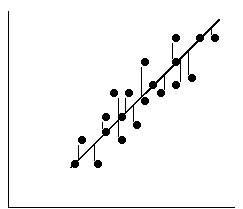
\includegraphics[height=.4\textheight]{regression.png}}

  \only<2>{
    \begin{displaymath}
      \min \sum (y_i-(ax_i+b))^2
    \end{displaymath}
    \vspace{1mm}
  }
  \vspace{1cm}
  \centerline{\gray{\footnotesize \url{http://www.upa.pdx.edu/IOA/newsom/pa551/Image255.gif}}}
  
\end{frame}

\begin{frame}
  \frametitle{Slope One : algorithm}

  Offline :
  \DontPrintSemicolon
  \begin{algorithm}[H]
    \For{chaque $I_i$, $I_j$}{
      $\mathcal{U} \gets \{\mbox{users who have expressed an opinion on } I_i, I_j \} $\;
      $\mbox{dev}_{i,j} \gets \frac{1}{\parallel\mathcal{U}\parallel}
      \sum_{u\in\mathcal{U}} (r_u(i) - r_u(j))$ \;
    }
  \end{algorithm}
  \bigskip
    Online (for $u$) :
  \DontPrintSemicolon
  \begin{algorithm}[H]
    $\mathcal{V} \gets \{ j \mid u \mbox{ has expressed an opinion on } I_j \} $\;
    $r_u(i) \gets \frac{1}{\parallel\mathcal{V}\parallel}
    \sum_{u\in\mathcal{V}} (\mbox{dev}_{i,j} - r_u(j))$ \;
  \end{algorithm}


\end{frame}

\begin{frame}
  \frametitle{Slope One : Regression}
  
  \vspace{1cm}
  \centerline{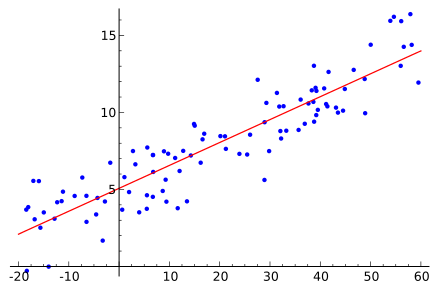
\includegraphics[height=.4\textheight]{linear-regression.png}}

  \vspace{1cm}
  \gray{\small "Linear regression" by Sewaqu - Own work. Licensed
    under Public domain via Wikimedia Commons -
    {\footnotesize\url{http://commons.wikimedia.org/wiki/File:Linear\_regression.svg\#mediaviewer/File:Linear_regression.svg}}}

\end{frame}

\begin{frame}
  \frametitle{Slope One : Regression}
  
  \vspace{1cm}
  \centerline{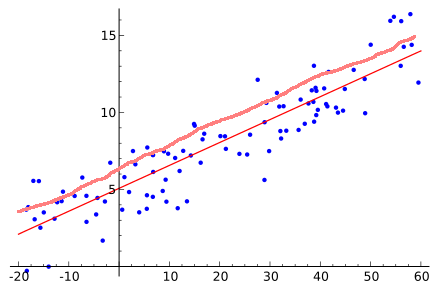
\includegraphics[height=.4\textheight]{linear-regression-2.png}}

\end{frame}


% ======================================================================
% Dimensionality Reduction

\begin{frame}
  \frametitle{Dimensionality reduction}

  SVD, typically $k=20\ldots 100$

  \only<1>{
    \begin{displaymath}
      M = U\Sigma V^*
    \end{displaymath}
  }
  \only<2>{
    \begin{displaymath}
      \begin{pmatrix}
        a_1 & \cdots & a_m
      \end{pmatrix}
      \begin{pmatrix}
        b_1 \\ \vdots \\ b_n
      \end{pmatrix} = \mathrm{scalar} 
    \end{displaymath}
  }
  \only<3>{
    \begin{displaymath}
      \begin{pmatrix}
        a_1 \\ \vdots \\ a_m
      \end{pmatrix}
      \begin{pmatrix}
        b_1 & \cdots & b_n
      \end{pmatrix} =
      \begin{pmatrix}
        c_{1,1} & \cdots & c_{1,n} \\
        \vdots & & \vdots \\
        c_{m,1} & \cdots & c_{m,n}
      \end{pmatrix}
    \end{displaymath}
  }
  \only<4>{
    \begin{displaymath}
      \begin{pmatrix}
        a_{1,1} & a_{1,2} & a_{1,3} \\
        \vdots & \vdots & \vdots \\
        a_{m,1} & a_{m,2} & a_{m,3}
      \end{pmatrix}
      \begin{pmatrix}
        b_{1,1} & \cdots & b_{1,n} \\
        b_{2,1} & \cdots & b_{2,n} \\
        b_{3,1} & \cdots & b_{3,n}
      \end{pmatrix} =
      \begin{pmatrix}
        c_{1,1} & \cdots & c_{1,n} \\
        \vdots & & \vdots \\
        c_{m,1} & \cdots & c_{m,n}
      \end{pmatrix}
    \end{displaymath}
  }
  \only<5>{
    \begin{displaymath}
      \begin{pmatrix}
        a_{1,1} & \cdots & a_{1,k} \\
        \vdots & & \vdots \\
        a_{m,1} & \cdots & a_{m,k}
      \end{pmatrix}
      \begin{pmatrix}
        c_{1,1} & \cdots & c_{1,n} \\
        \vdots & & \vdots \\
        c_{k,1} & \cdots & c_{k,n}
      \end{pmatrix} =
      \begin{pmatrix}
        c_{1,1} & \cdots & c_{1,n} \\
        \vdots & & \vdots \\
        c_{m,1} & \cdots & c_{m,n}
      \end{pmatrix}
    \end{displaymath}
  }
  
\end{frame}

\begin{frame}
  \frametitle{Challenges}

  \begin{itemize}
  \item How do we measure success?
  \item What are our features?
  \end{itemize}
\end{frame}

\begin{frame}
  \frametitle{Clustering}

  \begin{itemize}
  \item kNN \only<2>{\gray{$k$-Nearest Neighbor}}
  \item Curse of Dimensionality
  \item Scalability \only<2>{\gray{$10^7$ clients, $10^6$ objets}}
  \end{itemize}
\end{frame}

\begin{frame}
  \frametitle{The Codelab that Isn't}

  \phrase{crab is a candidate for inclusion in scikit-learn}

  \prevwork{\url{https://muricoca.github.io/crab/index.html}}
\end{frame}

% ======================================================================
% End

\begin{frame}
  \frametitle{Questions?}
  \centerline{\large\url{purple.com/talk-feedback}}
\end{frame}

\end{document}
